\section{Resultados} 
\label{posing:result}
%%%%%%%%%%%%%%%%%%%%%%%%%%%%%%%%%%%%%%%%%%%%%%%%%%%%%%%%%
\todo{No me gustan los apartados. Separa entre rendimiento y calidad}
\todo{Pasar todos los resultados al capítulo de resultados}

\todo{pasiva}
En esta sección se va a proceder a mostrar los resultados obtenidos por el algoritmo propuesto al transformar distintos modelos virtuales. Entre estos modelos, se incluyen modelos comerciales, otros procedentes de imágenes de pacientes reales o ejemplos básicos. Estos modelos representan una gran parte de la variabilidad a la que se pueda enfrentar el método propuesto. A continuación se enumeran los modelos utilizados:


\begin{table*}[h]


\centering

\caption{Complejidad de los modelos utilizados}
\label{tab:complex}
\begin{tabular}{|x{35mm}|x{20mm}|x{24mm}|x{20mm}|x{24mm}|}
\cline{2-5}
\multicolumn{1}{c}{ }
&
\multicolumn{2}{|c}{Malla superficial }
&\multicolumn{2}{|c|}{Malla volumétrica }
 \\
 \hline
\textbf{Modelo } 
& \textbf{Vértices }
& \textbf{Triángulos}
& \textbf{Nodos}
& \textbf{Tetraedros} \\ 

\hline
\emph{ZygoteBody}$^{TM}$ Masculino \cite{kelc2012zygote}            &1317862      &2601469   &553412 &2576779\\
\hline
\emph{ZygoteBody}$^{TM}$ Femenino \cite{kelc2012zygote}         &1468989     &2896011   &492646 &2314456\\ 
\hline
\emph{Anatomium} Masculino \cite{Anatomium}     &790461     &1570778    &767325 &3411170\\ 
\hline
\emph{Segmented Inner Organs}\cite{VoxelMan} &591265     &1184325    &242033  &1182485\\ 
\hline
Datos de pacientes reales     &31987       &63926   &82277  &346853\\ 
\hline
Modelo de barra con cuatro huesos  &2152     &4268    &8539 &39419\\ 
\hline



\end{tabular}

\end{table*}


% \begin{itemize}
%     \item \emph{ZygoteBody}$^{TM}$ Masculino \cite{kelc2012zygote}
%     \begin{itemize}
%         \item Vértices: 1317862
%         \item Triángulos: 2601469
%         \item Nodos: 553412
%         \item Tetraedros: 2576779
%     \end{itemize}
%     \item \emph{ZygoteBody}$^{TM}$ Femenino \cite{kelc2012zygote} 
%     \begin{itemize}
%         \item Vértices: 1468989
%         \item Triángulos: 2896011
%         \item Nodos: 492646
%         \item Tetraedros: 2314456
%     \end{itemize}
%     \item \emph{Anatomium} Masculino \cite{Anatomium}
%     \begin{itemize}
%         \item Vértices: 790461
%         \item Triángulos: 1570778
%         \item Nodos: 767325
%         \item Tetraedros: 3411170
%     \end{itemize}
%     \item \emph{Segmented Inner Organs}\cite{VoxelMan}
%     \begin{itemize}
%         \item Vértices: 591265
%         \item Triángulos: 1184325
%         \item Nodos: 242033
%         \item Tetraedros: 1182485
%     \end{itemize}
%     \item Datos de pacientes reales
%     \begin{itemize}
%         \item Vértices: 31987
%         \item Triángulos: 63926
%         \item Nodos: 82277
%         \item Tetraedros: 346853
%     \end{itemize}
%     \item Modelo de barra con cuatro huesos
%     \begin{itemize}
%         \item Vértices:  2152
%         \item Triángulos: 4268
%         \item Nodos: 8539
%         \item Tetraedros: 39419
%     \end{itemize}
% \end{itemize}

\begin{figure*}[h]%[b]%[b!ht]
  \centering
  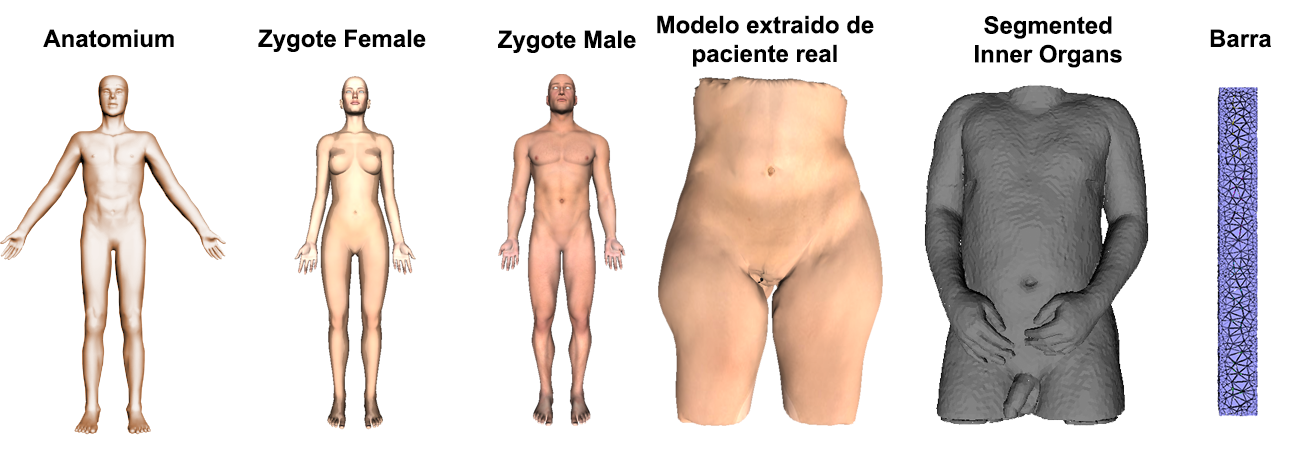
\includegraphics[width=0.90\textwidth]{IMG/modelos}
    \caption{Ejemplo de los modelos utilizados en los test.}
    \label{fig:models}
\end{figure*}

La tabla ~\ref{tab:complex} resume el tamaño de los modelos que se utilizarán y las mallas volumétricas asociadas a esos modelos mostrados en la figura \ref{fig:models}. Es necesario remarcar las dimensiones de los modelos anatómicos y las representaciones volumétricas en comparación con los tamaños habituales vistos en la sección de estado del arte (ver sección \ref{art:animation}). En ocasiones, estos modelos tienen una complejidad de un orden de magnitud superior a las mostradas en la bibliografía.

Con el objetivo de no necesitar un usuario con habilidades artísticas o conocimientos avanzados de anatomía, se han utilizado animaciones procedentes de la base de datos de \ac{MoCap} de la \emph{Carnegie Mellon University}~\cite{CMUMCD}.

El computador utilizado para realizar todos los test de la presente tesis se compone de un procesador \emph{Intel\textregistered i7-4820K @ 3.7GHz}, tarjeta gráfica \emph{GeForce GTX 770} y 16GB de memoria \acs{RAM}.


%\subsection{Proceso previo}
\subsection{Rendimiento}

Uno de los principales objetivos del algoritmo propuesto es que la selección de poses pueda ejecutarse interactivamente. Así pues, en el cauce de animación propuesto se han delegado las etapas más costosas computacionalmente a un proceso previo. Este proceso previo generará un conjunto de de datos que serán usados por la herramienta al seleccionar el modelo virtual asociado. Estos datos solo son necesarios crearlos una vez por modelo. En las pruebas realizadas, el tiempo de procesador nunca ha excedido más de siete minutos. 


Hay que destacar que los modelos con los que se ha trabajado no están exentos de problemas. Por una parte, en ambos modelos de \emph{ZygoteBody}$^{TM}$ presentan auto-colisiones y se puede encontrar multitud de colisiones entre distintos tejidos. Además, zonas anatómicas muy próximas (p. ej. la axila) pueden resultar conflictivas como se puede observar en la figura \ref{fig:zygoteproblems}. 

Por otra parte, muchos de los procedimientos médicos se realizan en áreas localizadas, por lo tanto, muchas de las imágenes médicas disponibles no representan completamente el modelo anatómico del paciente. El algoritmo propuesto es capaz de tratar con información incompleta como podemos observar en la figura \ref{fig:patient} donde se muestra un modelo construido a partir de imágenes médicas reales.

\begin{figure}[h]
   \centering
    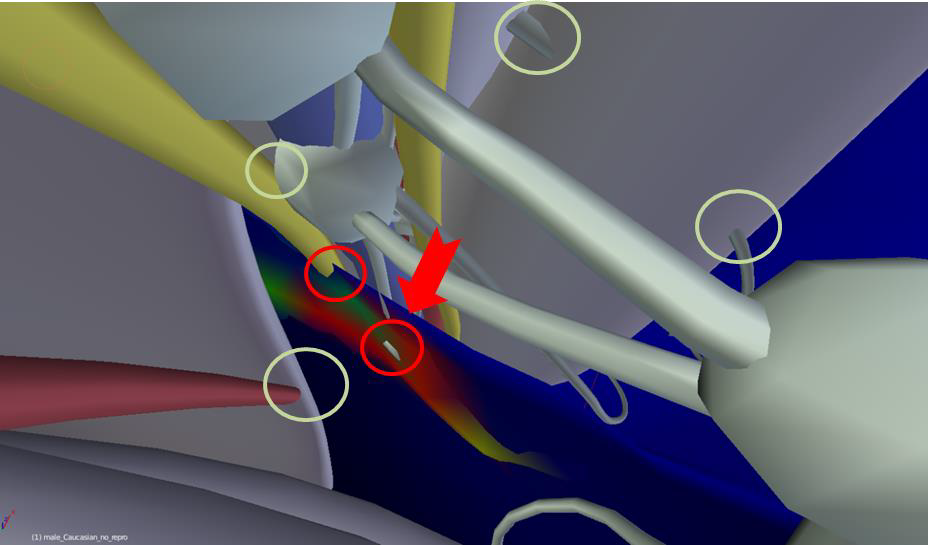
\includegraphics[width=0.5\textwidth]{IMG/zygoteproblems.png}
    \caption{Axila del modelo \emph{ZygoteBody}$^{TM}$ Masculino. Con círculos amarillos se observa colisiones entre diferentes tejidos. Los círculos rojos representan colisiones con el tejido de la piel  }
   \label{fig:zygoteproblems}
\end{figure}


%%%%%%%%%%%%%%%%%%%%%%%%%%%%%%%%%%%%%
\begin{figure}[h]
   \centering
    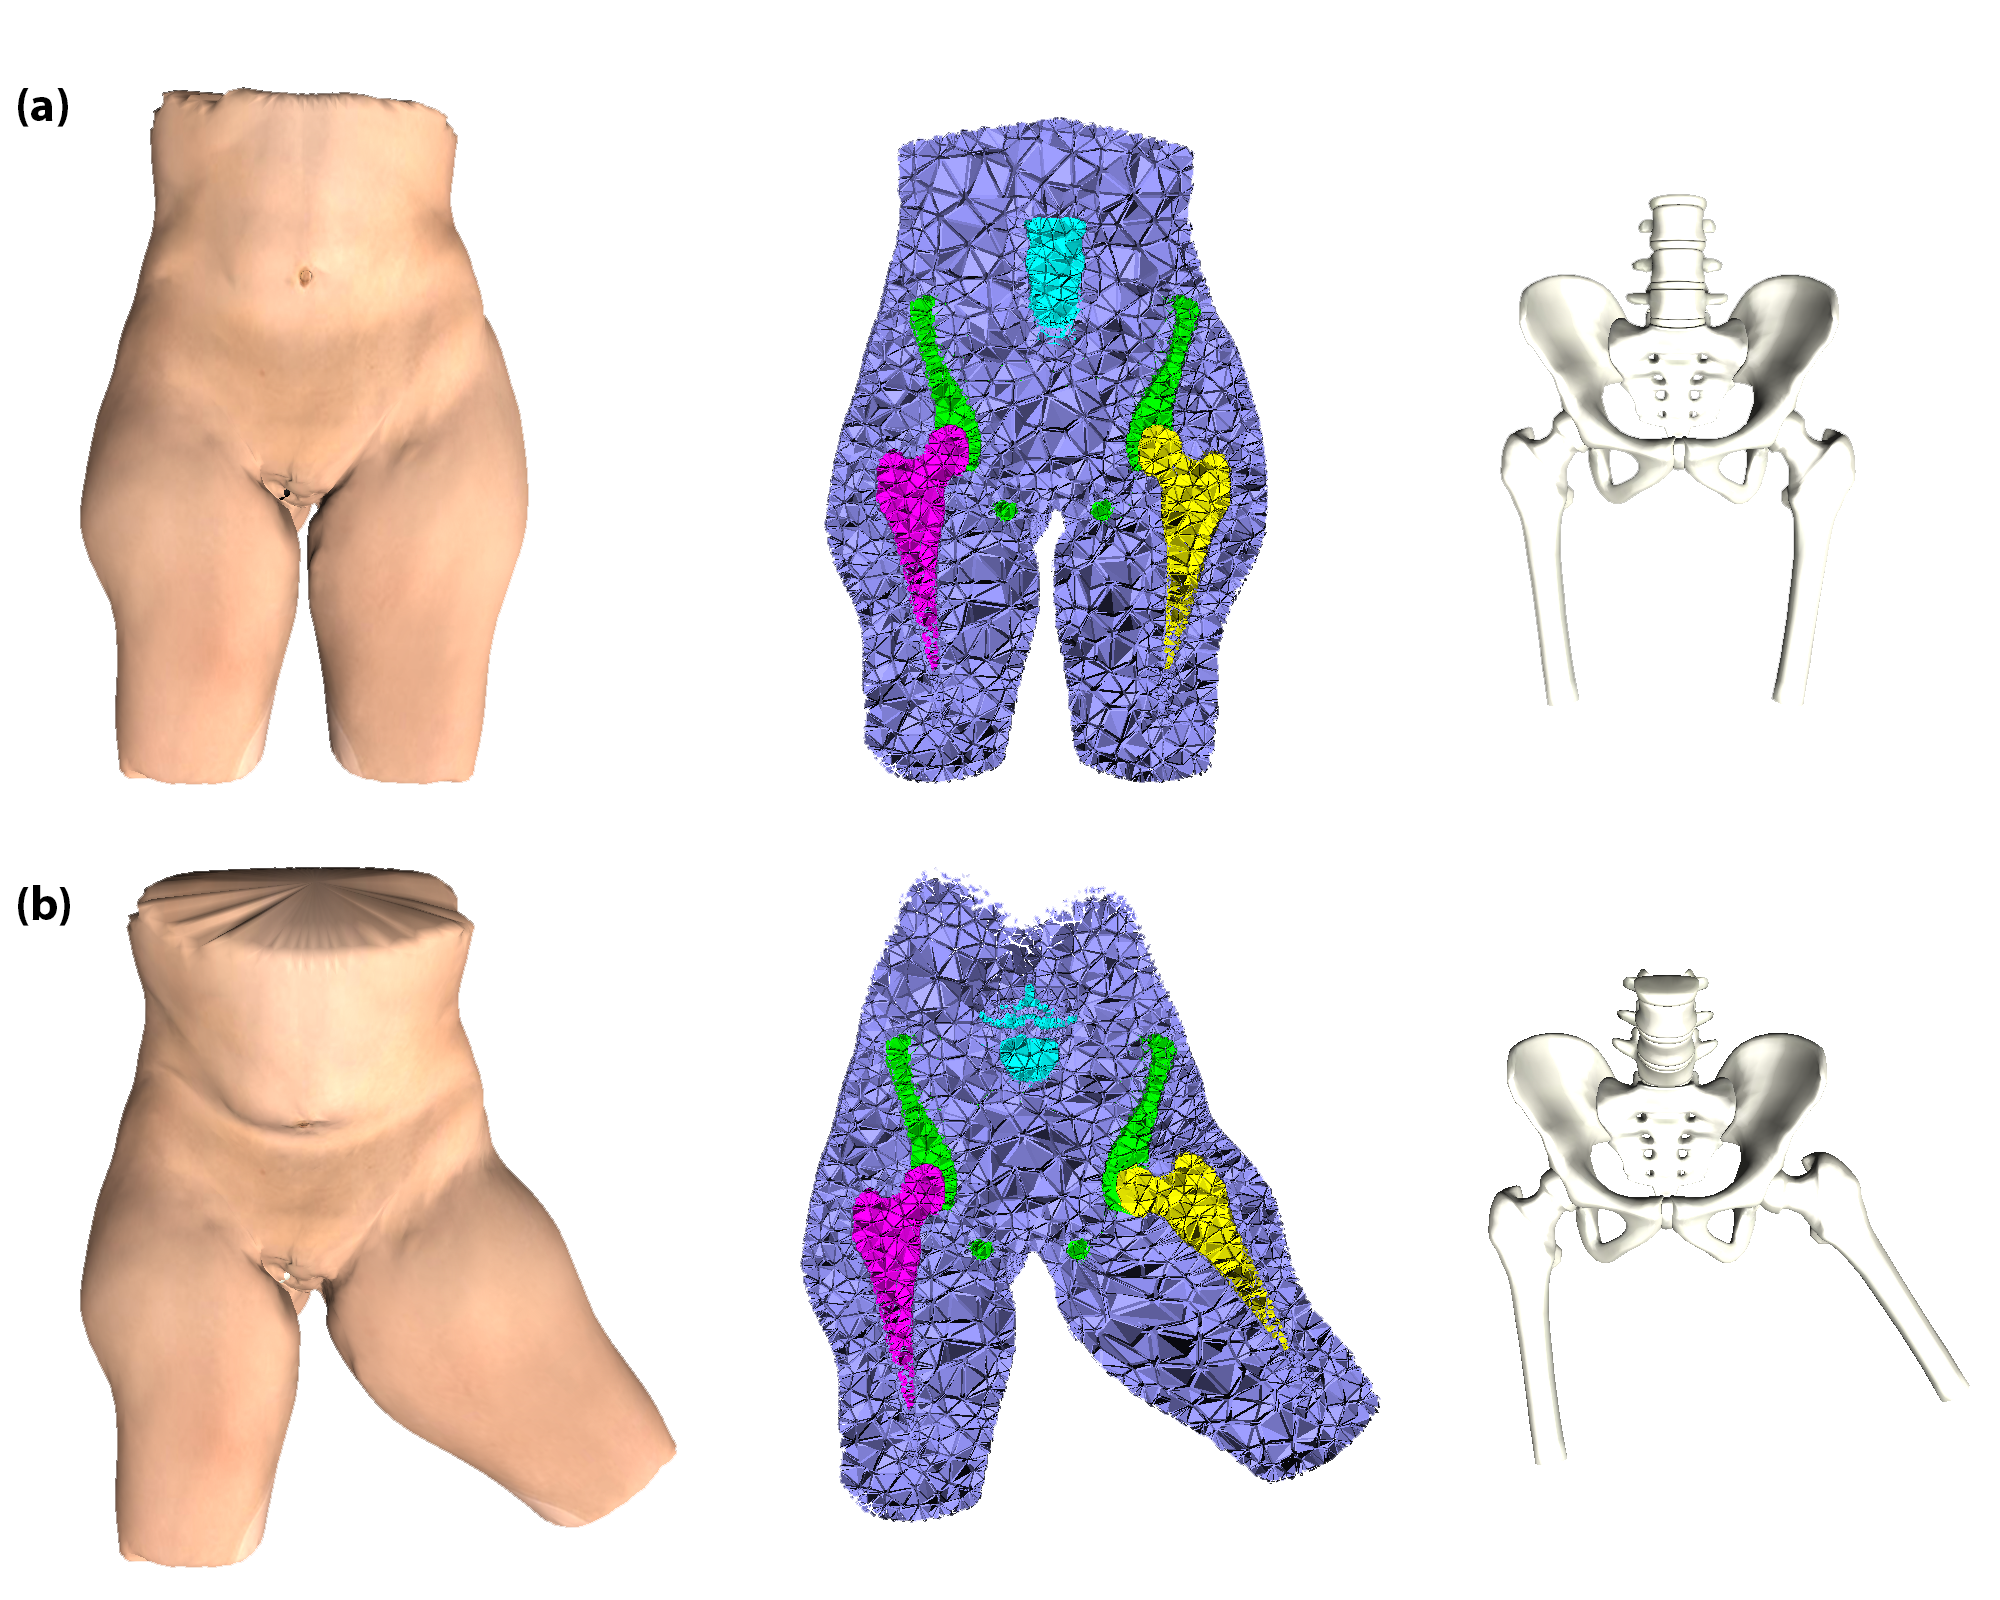
\includegraphics[width=0.5\textwidth]{IMG/patient.png}
    \caption{ La fila (a) muestra el paciente virtual construido a partir de datos de paciente real y se encuentran en posición de reposo. El algoritmo de posicionamiento permite modificar la pose de estos datos.
    }
   \label{fig:patient}
\end{figure}
%

Debido a la necesidad de que el algoritmo resulte robusto frente a los problemas comentados, se ha procedido a añadir diferentes ajustes en el algoritmo propuesto en varias de sus etapas.

En la etapa de \emph{volumetrización} (sec. \ref{posing:volumetrizacion}) se ha modificado la voxelización  para borrar los \emph{vóxeles} etiquetados por el borde de la piel. Por tanto, en la figura \ref{fig:voxelizacion}.c se puede observar que los \emph{vóxeles} marcados como piel son etiquetados de nuevo como vacío con el objetivo de no crear tetraedros entre zonas próximas pero no interconectadas. En la figura \ref{fig:volsol} se puede observar la diferencia en la malla volumétrica. En la columna de la izquierda se muestra la \emph{voxelización} de la axila sin quitar los \emph{vóxeles} de la piel, lo que se traduce en una conexión entre zonas próximas. En la columna de la derecha se puede observar que la zona de la axila esta correctamente separada.

\begin{figure}[h]
   \centering
    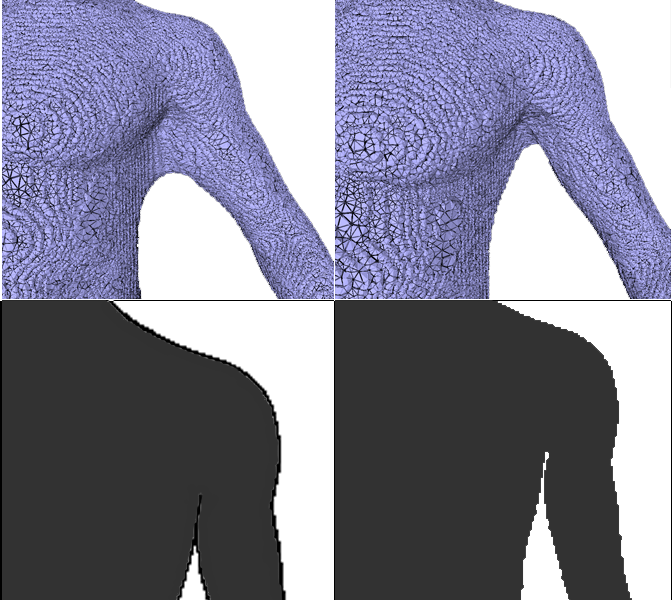
\includegraphics[width=0.45\textwidth]{IMG/volumetrizacion2.png}
    \caption{
    \emph{Volumetrización} de la zona de la axila. Columna izquierda muestra el problema de no eliminar los \emph{vóxeles} etiquetados como piel, en la columna de la derecha se resuelve el problema }
\label{fig:volsol}
\end{figure}


Con esta modificación se resuelve problemas de interconexión entre zonas no conectadas, aunque podría generar que se pueda encontrar tejidos que no están dentro de la malla volumétrica. Esta solución genera un problema  adicional al crear situaciones donde se puedan encontrar ciertos tejidos fuera de la piel. Debido a esto se ha propuesto una modificación adicional de la etapa mapeado (ver sección \ref{posing:Mapeado}) para resolver este problema. Aprovechando la estructura espacial que proporciona la \ac{tabla hash}, aunque el vértice no esté dentro de ningún tetraedro, es fácil buscar el tetraedro más cercano en las subdivisiones vecinas para asociarle con él. 
Con esta modificación, en el caso concreto del modelo \emph{ZygoteBody}$^{TM}$ Masculino, alrededor de un 4.6\% de los vértices se encontrarían fuera de la malla volumétrica. 
Estos vértices no afectan de manera determinante en el proceso de mapeado. En este caso, el tiempo de mapeado es 36,35 segundos utilizando la \ac{tabla hash} como método de búsqueda. Este tiempo es muy pequeño si se compara con el tiempo que tardaría el proceso de mapear usando la técnica de fuerza bruta, que sería de 4 horas y 55 minutos para relacionar 1277325 de vértices a 2584115 de tetraedros en el caso del mismo ejemplo.  En la tabla \ref{tab:bruteforce} se muestra una comparación entre los tiempos empleados en mapear los distintos tejidos del \emph{ZygoteBody}$^{TM}$ Masculino con su malla volumétrica. La complejidad de la malla de tetraedros se puede consultar en la figura \ref{fig:models}. Los modelos más complejos obtienen datos similares que se sitúan en torno a los cinco a siete minutos.


       
        
\begin{table*}[h]

\begin{threeparttable}
\centering

\caption{Comparación de tiempos de mapeado entre la técnica de \emph{Spatial Hashing} y fuerza bruta. }
\label{tab:bruteforce}
\begin{tabular}{|c|c|x{25mm}|x{25mm}|x{25mm}|}

\hline
\textbf{Modelo} & \textbf{Vértices} & \textbf{Vértices  huérfanos (\%)}  & \textbf{Spatial Hashing (ms)} & \textbf{Fuerza bruta (ms)} \\ 
\hline
Piel             &32748      &89.81   &10678* &547967\\
\hline
Músculos         &311600     &2.02    &12157* &4088365\\ 
\hline
S. nervioso      &379008     &1.41    &12814* &5140770\\ 
\hline
Tejido conectivo &168343     &0.68    &7881*  &2210942\\ 
\hline
S. linfático     &5324       &5.66    &5456*  &702087\\ 
\hline
S. circulatorio  &380302     &4.29    &11541* &5008874\\ 
\hline
\textbf{TOTAL}   &1277325    &4.6     &36357  &$17.7*10^6$ \\
\hline

\end{tabular}
\begin{tablenotes}
      \small
      \item * La creación de la \ac{tabla hash} esta incluida en cada medición (4834 ms). El tiempo total no puede ser calculado directamente sumando todos los valores de la columna.
    \end{tablenotes}

\end{threeparttable}
\end{table*}


Para finalizar de describir el proceso previo del algoritmo, a continuación se muestra la tabla \ref{tab:pre_pro} dónde se pueden consultar el tiempo empleado de cada etapa utilizando algunos de los modelos propuestos. 

%\todo{meter todos los valores significativos de configuración}

%Los valores de configuración para las distintas etapas son las siguientes:
La volumetrización no se hará en una caja contenedora más grande de tamaño 250x700x120. En cuanto a la función de similaridad empleada en la técnica de \emph{skinning} \ac{COR}, el valor de $\sigma$ que se utiliza es $0.1$. El \emph{ratio de Poisson} se estableció en 4.999 y el \emph{módulo de Young} en 0.01.




\begin{table*}[!h]
\centering
\caption{Tiempo en milisegundos utilizado por cada etapa. ZM es Zygote Masculino, ZF es Zygote Femenino, A es Anatomium y \ac{COR} es la etapa de calcular los centros de rotación (sec. \ref{posing:Poses}).}
\begin{tabular}{|c|c|c|c|c|c|}
\hline
\textbf{Modelo} & \textbf{Rigging} & \textbf{Volumetrización} & \textbf{Pesado} & \textbf{Mapeado} & \textbf{COR }  \\ 
\hline
ZM  & 32698 & 69044 & 11762  & 51160   & 138005 \\ 
\hline
ZF  & 33251 & 63401 & 9171  & 71635   & 208886  \\ 
\hline
A   & 31891 & 120465 & 23318 & 44521  & 115214\\ 
\hline
\end{tabular}
\label{tab:pre_pro}
\end{table*}


En cuanto a la etapa de selección de poses, esta debe ser interactiva al ser necesaria la intervención de un usuario para supervisar la deformación de los tejidos. Además, es importante remarcar que el algoritmo propuesto puede manejar una gran cantidad de vértices y tetraedros como se puede observar en los datos de la figura \ref{fig:models}. En la tabla \ref{tab:inter} se muestra el rendimiento del método seleccionado (\ac{COR}) frente a los dos métodos clásicos más conocidos en la literatura que son \ac{LBS} y \ac{DQS}. Como se puede observar, el rendimiento entre las diferentes técnicas son muy similares. La tabla muestra los valores máximos y mínimos de imágenes por segundo que es capaz de generar el algoritmo utilizando un ciclo de caminado para animar al modelo virtual.
%
\begin{table}[h]
\centering
\caption{Valores máximos y mínimos de imágenes por segundo durante el ciclo de caminado en la etapa de \emph{selección de poses} }
\begin{tabular}{|c|c|c|c|}
%\multirow{2}{*}{\textbf{Model}} & \multicolumn{2}{c}{\textbf{Interactive stage}} & \multirow{2}{*}{\textbf{Optimization}} \\
\hline
\textbf{Modelo}&\textbf{LBS} &\textbf{DQS} &\textbf{COR} \\ 
\hline
ZM  & 111-90 & 100-90 & 100-76\\ 
\hline
ZF  & 76-60  & 66-52   & 60-50 \\ 
\hline
A   & 166-142 & 166-125 & 142-100\\ 
\hline
\end{tabular}
\label{tab:inter}
\end{table}



%\subsection{Selección de poses}
\subsection{Aspecto visual} \todo{Hay otro tipo de nombre para esta sección?}
A continuación, en esta sección se van a comparar los resultados visuales que produce el algoritmo utilizando el método de \emph{skinning} \ac{COR} y las otras dos técnicas más utilizadas. 


%La etapa de selección de poses del algoritmo incluye la fase de \emph{skinning} para los vértices de los tetraedros y la consecuente deformación que es transferida a los tejidos del modelo virtual. 
Inicialmente, para mostrar de manera simple las diferencias visuales que se generan a través de las tres técnicas anteriormente citadas, se va a utilizar un modelo simple de un prisma rectangular con cuatro huesos virtuales en su interior. Este modelo por su simplicidad se utilizará para mostrar los resultados de rotaciones y giros para que se pueda visualizar de forma directa las diferencias entre técnicas utilizadas. En la figura \ref{fig:bar_bending} se pueden observar las diferencias visuales del método seleccionado (\ac{COR}) frente a los dos métodos clásicos más conocidos en la literatura que son \ac{LBS} y \ac{DQS}. En cuanto a las rotaciones, se puede apreciar que en el caso de \ac{LBS} la articulación pierde volumen (llamado normalmente \emph{collapsing elbows}), sin embargo, en \ac{DQS} se puede observar un aumento de volumen (se utiliza la denominación \emph{joint-bulging effect}). Respecto a los giros, es conocido que la técnica \ac{DQS} solventa el problema de \ac{LBS} donde la interpolación de los vértices se realiza de forma lineal produciendo el efecto \emph{candy-wrapper}. Así que, la técnica \ac{COR} es más robusta a cambios de volumen en rotaciones y además maneja adecuadamente los giros de las articulaciones. En esta figura se utilizan los tetraedros como referencia visual mostrando con los colores el pesado mostrado las diferentes influencias de los huesos virtuales. Se ha usado un código de colores, donde el color azul resultar ser los huesos impares que tienen influencia de 1 y el color rojo es donde los huesos pares tienen influencia de 1. Con este código de colores se puede observar las transiciones entre huesos.

\begin{figure*}[h]%[b]%[b!ht]
  \centering
  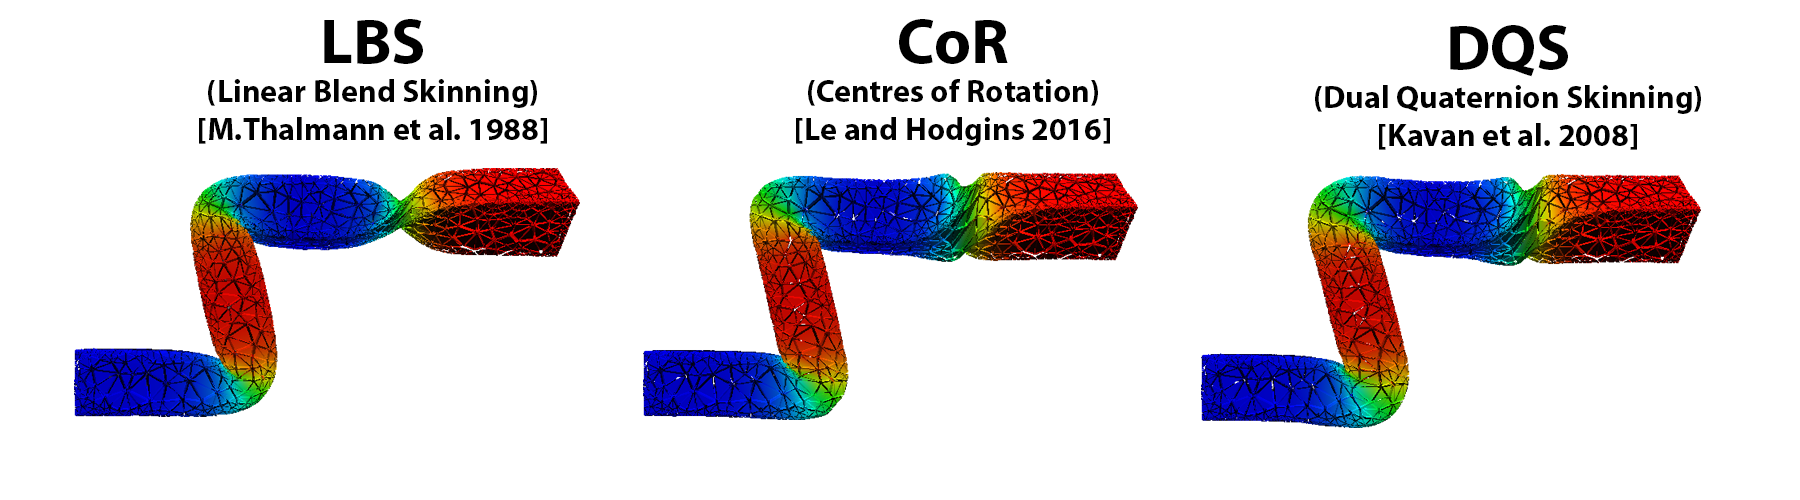
\includegraphics[width=0.90\textwidth]{IMG/BarraCoR}
    \caption{Deformación del modelo de barra por las 3 técnicas. Primera rotación de 100º, segunda rotación de -100º y un giro de 135º.}
    \label{fig:bar_bending}
\end{figure*}
%%%%%%%%%%%%%%%%%%%%%%%%%%%%%%%%%%%%%

Una vez ilustradas las diferencias de manera teórica, a continuación se mostrarán las diferencias entre las distintas técnicas de \emph{skinning} utilizando los modelos anatómicos. En las siguientes figuras, se utilizará diferentes posturas de los modelos anatómicos para mostrar las diferencias en los resultados que producen cada uno de los métodos al deformar el paciente virtual.

En la figura \ref{fig:thigh_bending} se muestra una rotación de la articulación de la pierna. Las zonas perceptibles de producir artefactos son la zona superior del muslo en la zona inguinal y el glúteo. En esta imagen se puede observar que tanto la zona inguinal y el glúteo con la técnica \ac{LBS} produce una pérdida de volumen. En el caso de utilizar \ac{DQS}, se aprecia el aumento de volumen predicho para esta técnica. Sin embargo, la técnica \ac{COR} da como resultado un compromiso entre ambas técnicas. La imagen se acompaña con el tejido muscular en reposo como referencia. Se acompaña una deformación de los tejidos circulatorio y nervioso como ejemplo de tejidos internos del modelo. En este ejemplo en concreto, las diferencias visuales entre técnicas de estos dos tejidos es mínima al ser estructuras filiformes. 





% %%%%%%%%%%%%%%%%%%%%%%%%%%%%%%%%%%%%%
\begin{figure*}[h]%[b]%[b!ht]
  \centering
  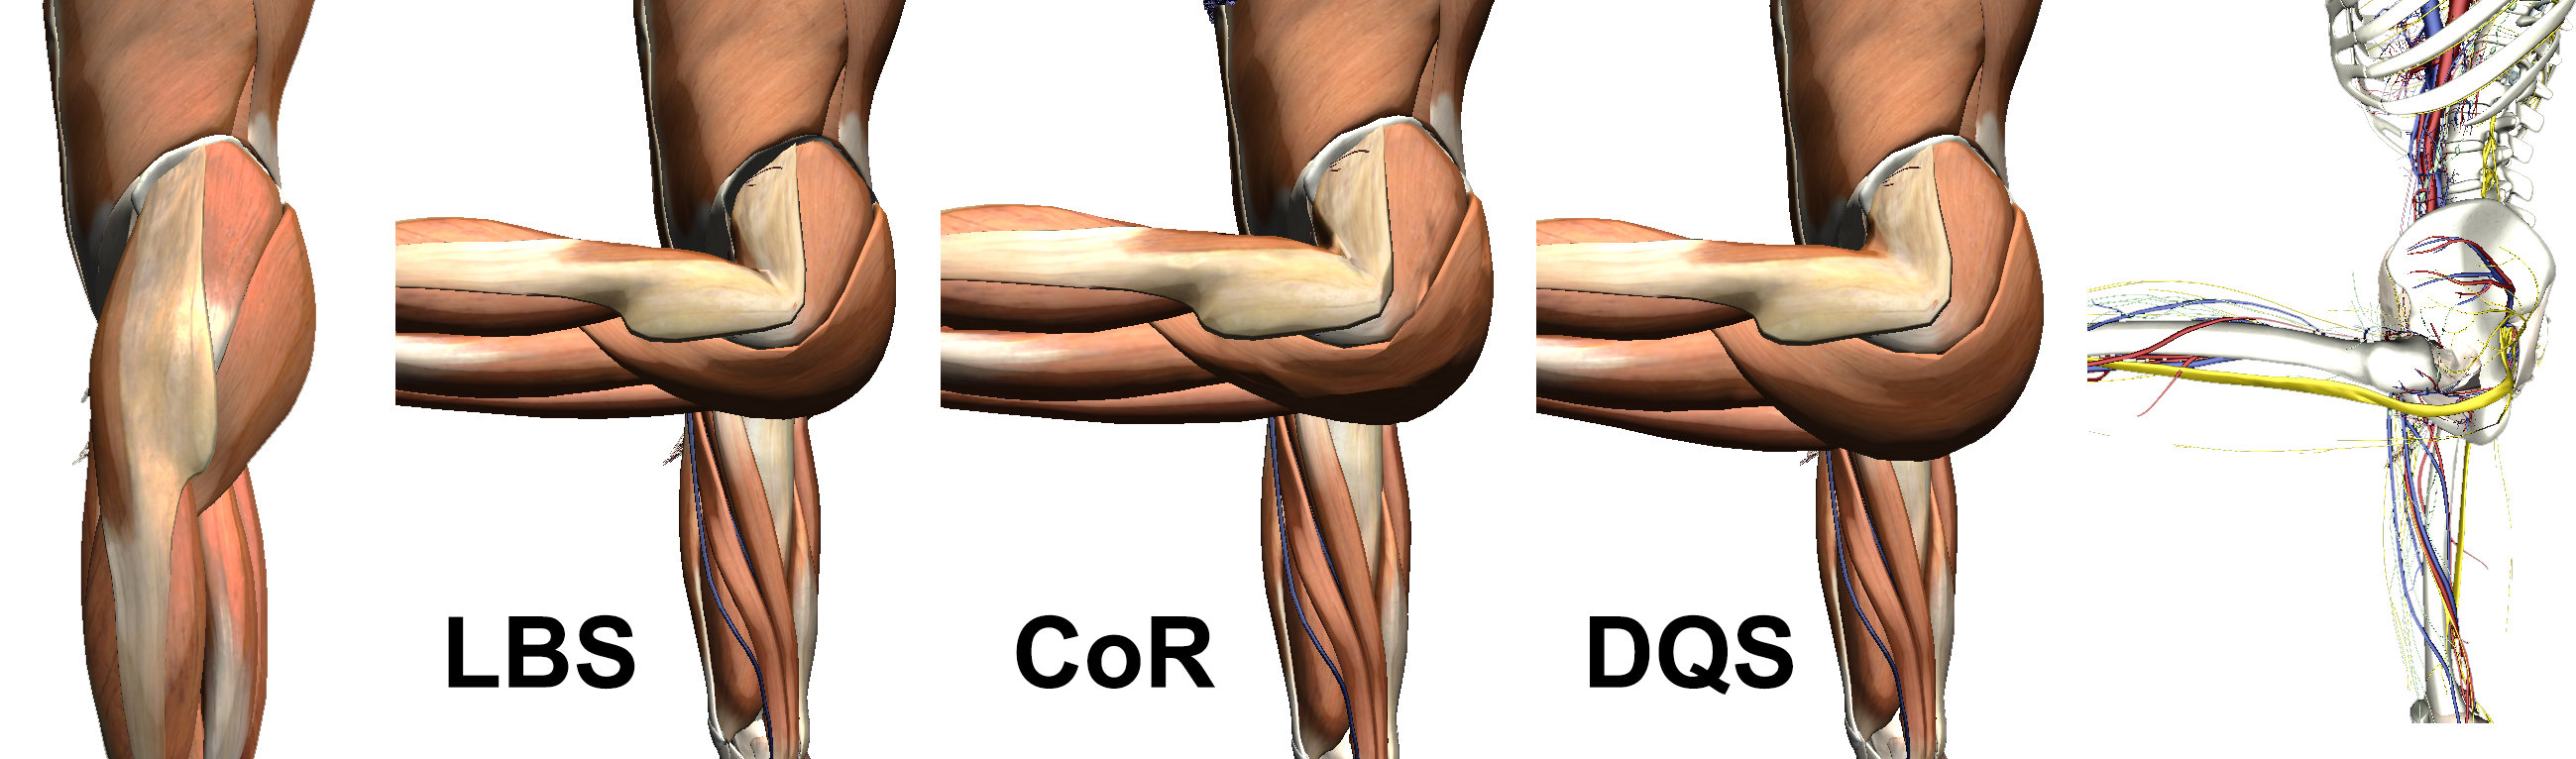
\includegraphics[width=0.90\textwidth]{IMG/compculo}
    \caption{ Deformación de una pierna. Izquierda: posiciones de los músculos en reposo; en el medio se muestran la pierna rotada usando las 3 técnicas de \emph{skinning} (\ac{LBS} pierde volumen tanto en el gluto como en la zona inguinal, \ac{DQS} añade volumen y \ac{COR} suaviza esos defectos; a la derecha podemos ver otros tejidos deformados.}
    \label{fig:thigh_bending}
\end{figure*}

\todo{más ejemplos aqui}
%%%%%%%%%%%%%%%%%%%%%%%%%%%%%%%%%%%%%




\del{Con los resultados obtenidos, se puede afirmar que el algoritmo propuesto obtiene deformaciones visualmente realistas y es capaz de realizarlas en tiempo de ejecución delegando las etapas más pesadas a un proceso previo.}

Finalmente, en la imagen \ref{fig:run1} se muestran resultados adicionales del uso del algoritmo con la técnica de \emph{skinning} \ac{COR} en los modelos \emph{ZygoteBody}$^{TM}$ Masculino y Femenino en diferentes situaciones.

%%%%%%%%%%%%%%%%%%%%%%%%%%%%%%%%%%%%%
\begin{figure*}%[h]%[b]%[b!ht]
   \centering
   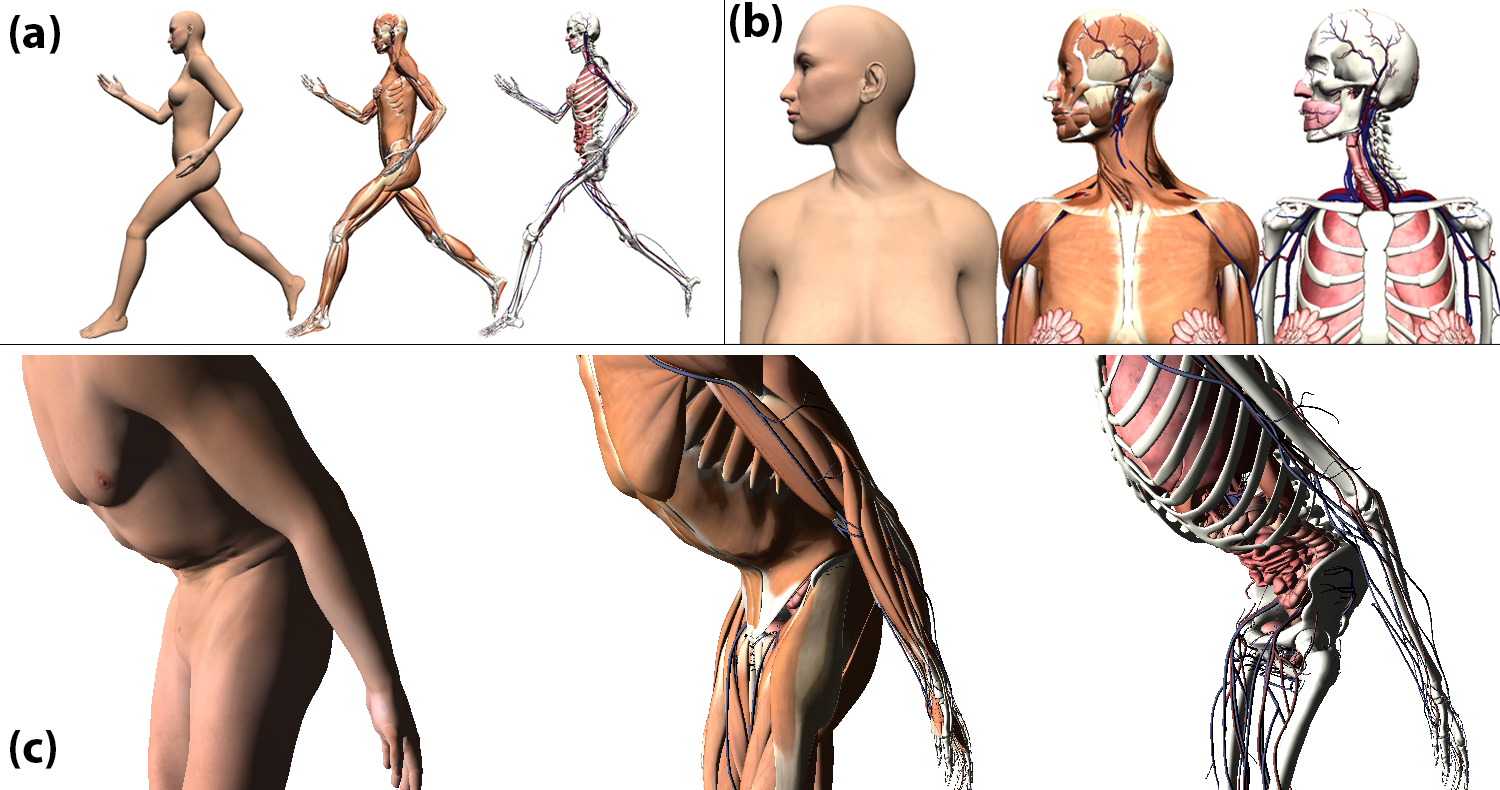
\includegraphics[width=0.90\textwidth]{IMG/examples}
    \caption{Resultados obtenidos utilizando \ac{COR}. (a): fotograma del ciclo de correr en el modelo ZF. (b): Cuello girado del modelo ZF. (c): Zona abdominal flexionada del modelo ZM.}
    \label{fig:run1}
\end{figure*}
%%%%%%%%%%%%%%%%%%%%%%%%%%%%%%%%%%%%%

\subsection{Optimización}
\label{posing:optimizacion}
Las deformaciones resultantes de la etapa anterior dan como resultado poses visualmente creibles en la mayoría de los casos. 
Aun así, se ha incluido la fase de optimización que permita al usuario deformar el paciente virtual con una técnica basada en físicas aunque no se dispongan de las descripciones mecánicas. A continuación, se mostraran la comparación de los resultados obtenidos y una evaluación para conocer si el usuario prefiere esta fase adicional frente a la solución geométricas.

La fase de \emph{skinning} basada en \ac{COR} solventa de forma efectiva los problemas típicos de las técnicas basadas en \ac{LBS} y de \ac{DQS}. Aún así, en algunas circunstancias se ha detectado un cambio no deseado que se traduce visualmente en un aumento o disminución de volumen. 
La técnica \ac{COR} no puede asegurar la conservación de volumen tal y como lo hacen las técnicas basadas en física debido a que no se tiene en cuenta. En esta sección, se va a comparar \ac{COR} con el resultado físico generado por la optimización. Debido a que no se puede asegurar una apropiada descripción mecánica de los tejidos, el objetivo de esta optimización es garantizar la conservación del volumen.  
Se ha propuesto utilizar la formulación \ac{FEM} co-rotacional para resolver el problema estático considerando un material lineal, isotrópico y homogéneo. Se ha escogido el módulo de \emph{Young}  intentado mejorar la estabilidad del sistema. Para ello, se han analizado distintas matrices de coeficientes del sistema, obtenidas a partir de distintos valores del módulo de \emph{Young}, quedándose con el valor que daba como resultado la matriz de coeficientes con menor número condicionante. En la mayoría de los casos probados, solo se necesitaba una iteración al resolver el sistema. Los resultados obtenidos con más iteraciones eran prácticamente indistinguibles. 
 
%  Besides, the deformations are measured using the \emph{Cauchy} strain tensor. The boundary conditions, needed to solve the steady-state problem, are given by the positions of the vertices labelled as bones. The co-rotational formulation calculates the internal forces caused by the deformations in a non-rotated configuration. Then, the internal forces are rotated again into the final configuration \cite{Muller2004}. The algorithm needs to compute the element rotations in the final configuration. For this purpose, the solution is refined iteratively. The elastic used model can be tuned with two parameters: the \emph{Poisson ratio}  and the \emph {Young module}. The \emph{Poisson ratio} controls the volume conservation and it should take a value close to 0.5 (the real value has to be lower to ensure numeric stability). Since the material is homogenous, this value has no impact on the outcome. 

La figura \ref{fig:anatomium} ilustra un ejemplo de cómo la técnica basada en la formulación \ac{FEM} soluciona alguna de los problemas de volumen que aparece con las otras técnicas. Sin embargo, debido a que la técnica \ac{COR} muestra buenos resultados se ha procedido a comprobar la hipótesis según la cual la optimización es elegida por los usuarios frente a la técnica geométrica.
 
\begin{figure}[h]%[b]%[b!ht]
   \centering
   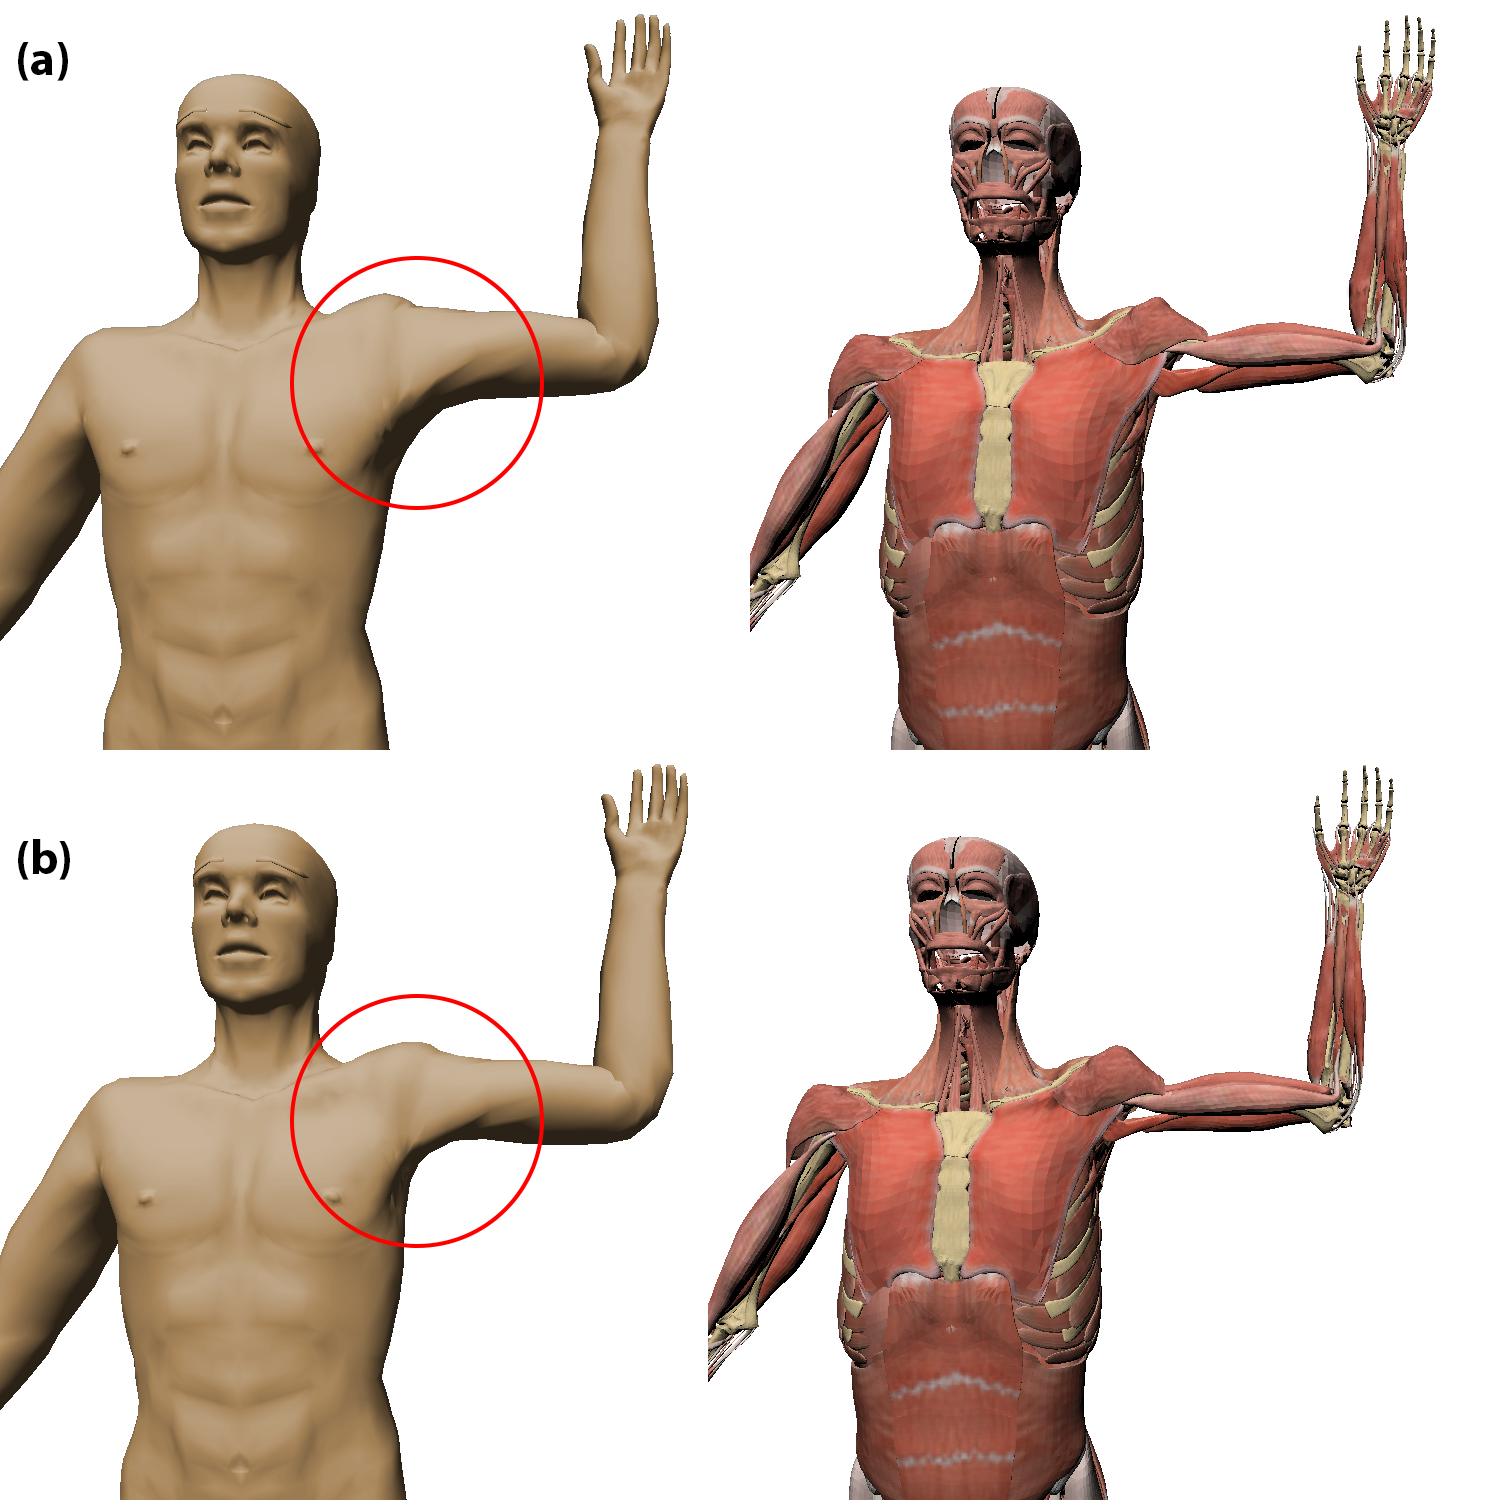
\includegraphics[width=0.45\textwidth]{IMG/AntCOR}
    \caption{ Comparación entre \ac{COR} (a) y el método \ac{FEM} (b)diseñado para conservar el volumen. \ac{COR} incrementa ligeramente el volumen en la zona de la axila.}
    \label{fig:anatomium}
\end{figure}
 
Para probar esta hipótesis, se ha procedido a realizar una encuesta entre distintos usuarios. Un total de 16 sujetos han participado en la encuesta que se puede encontrar en los anexos \label{anexo:cuestionario1} y \label{anexo:cuestionario2}\todo{Metemos la gráfica de la otra encuesta?}. En total, han sido 2 mujeres y 14 hombres, con una edad comprendida entre los 20 y los 52; donde 13 de ellos han declarado profesionales de informática gráfica. En estas encuestas, se ha pedido a los participantes que valoren el realismo presentado en unas imágenes estáticas. Estos sujetos debían contestar a una serie de preguntas, basándose en una escala de tipo  \emph{Likert} comprendida entre los valores 1 y 8. Las imágenes muestran seis posiciones diferentes y varios modelos y tejidos, donde la mitad de ellos han sido creados con la optimización \ac{FEM} y la otra mitad con la técnica \ac{COR}. Primero se ha mostrado la imagen de referencia para cada deformación y después se presenta de manera aleatoria las deformaciones con \ac{FEM} y \ac{COR}.

\new{ Al no seguir una distribución normal, se han comparado los resultados obtenidos usando la prueba de los rangos con signo de Wilcoxon no paramétrica para comparar el rango medio de dos muestras relacionadas y determinar si existen diferencias entre ellas. Con el resultado obtenido (\emph{p-value} $> 0.9$ intervalo de confianza) no se puede confirmar que los usuarios encuentren diferencias significativas entre ambos modelos. En la figura \ref{fig:stat} se muestra los resultados de la encuesta en una representación con dos diagramas de cajas y bigotes. }
%

%

\begin{figure}[h]%[b]%[b!ht]
   \centering
   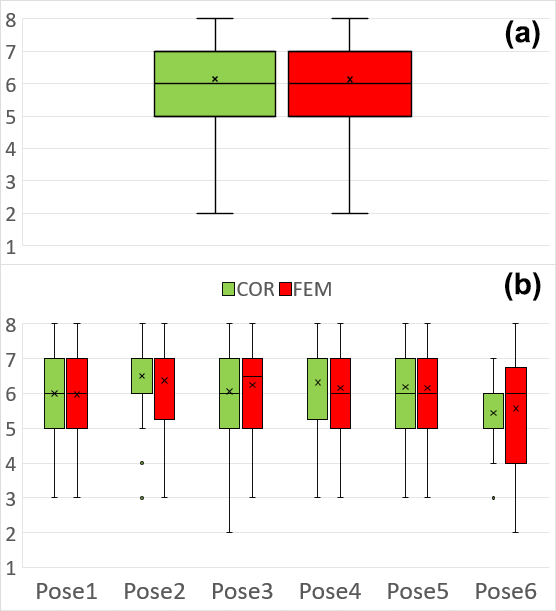
\includegraphics[width=0.45\textwidth]{IMG/boxplot}
    \caption{ Diagramas de cajas de bigotes comparando los resultados de la encuesta. Diagrama (a) muestra el resultado global, mientras el diagrama (b) compara el resultado obtenido por cada pose diferente.}
\label{fig:stat}
   \end{figure}

%%%%%%%%%%%%%%%%%%%%%%%%%%%%%%%%%%%%%

\subsection{Animación de representaciones volumétricas}
\label{posing:animvol}

\begin{figure*}[!ht]%[b]%[b!ht]
   \centering
   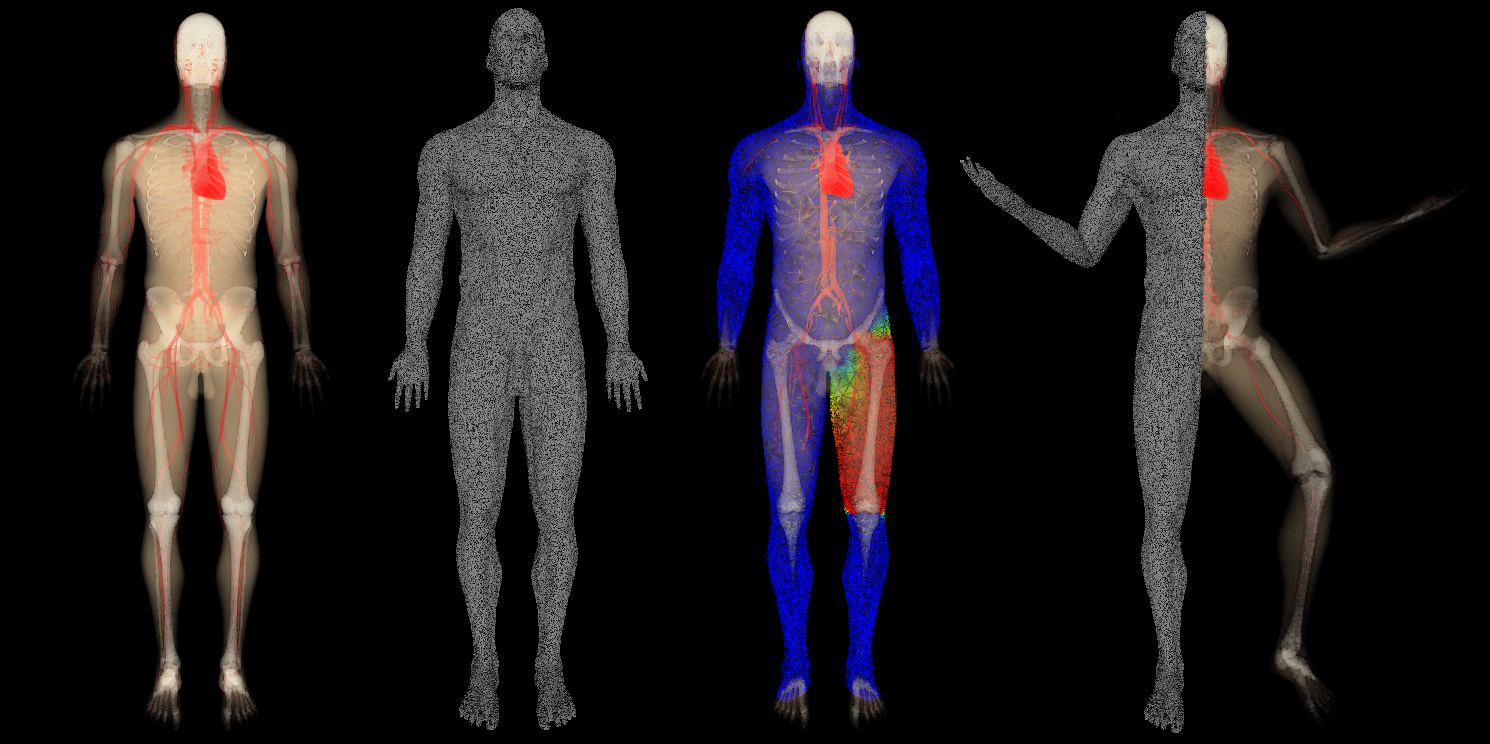
\includegraphics[width=0.90\textwidth]{IMG/Volumetric}
    \caption{Proceso de animación para modelo volumétrico. De izquierda a derecha: (1) modelo volumétrico en reposo, (2) malla de tetraedros generada, (3) malla de tetraedros representando el peso del fémur como ejemplo (rojo significa influencia cerca de 1, azul influencia 0) y (4) malla de tetraedros superpuesta al modelo volumétrico deformado. }
    \label{fig:volEx}
\end{figure*}
\todo{explica el por qué: el campo de desplazamientos, me he traido esto para inspirarme}

Como se puede leer en la sección 
\ref{posing:method}, el algoritmo se basa en el cálculo de un campo de desplazamientos continuo (ver sec. \ref{posing:volumetrizacion}) %\todo{si no es continuo todo lo que dices a continuación no sirve}
en el interior del paciente virtual que permita transformar sus estructuras internas. Esto permite deformar los tejidos de forma independiente y, aun así, garantizar que estos se muevan solidariamente, asegurando que no se produzcan colisiones. Se ha decido deformar los tetraedros y posteriormente interpolar el movimiento a los vértices usando las coordenadas baricéntricas, en lugar de transferir los pesos calculados (ver sec. \ref{posing:Pesado}) de los tetraedros a los vértices interiores de los tejidos y calcular el movimiento posteriormente.
De esta forma, el campo de desplazamientos definido se puede usar para transformar tanto vértices de representaciones superficiales como \emph{vóxeles} en modelos volumétricos. 


\new{En la figura \ref{fig:volEx} se muestra los pasos para obtener una deformación de una representación volumétrica. En primer lugar, se genera tetraedriza el modelo utilizando la misma técnica explicada en la sección \ref{posing:volumetrizacion}  y se calculan los pesos como se detalló en la sección \ref{posing:pesado}. A partir de la malla de tetraedros, se definen una serie de \emph{píxeles} dentro de cada tetraedro en la posición deformada. Se mapean con la configuración de reposo utilizando la transformación inversa del campo de desplazamiento. Para ello, se itera sobre cada caja contenedora de la \ac{tabla hash} y se utilizan las coordenadas baricéntricas. Este proceso al ser fácilmente paralelizable en \ac{GPU} permite que se pueda \emph{renderizar} en tiempo real.}
%


%%%%%%%%%%%%%%%%%%%%%%%%%%%%%%%%%%%%%
\begin{figure}[!ht]%[h]%[b]
   \centering
   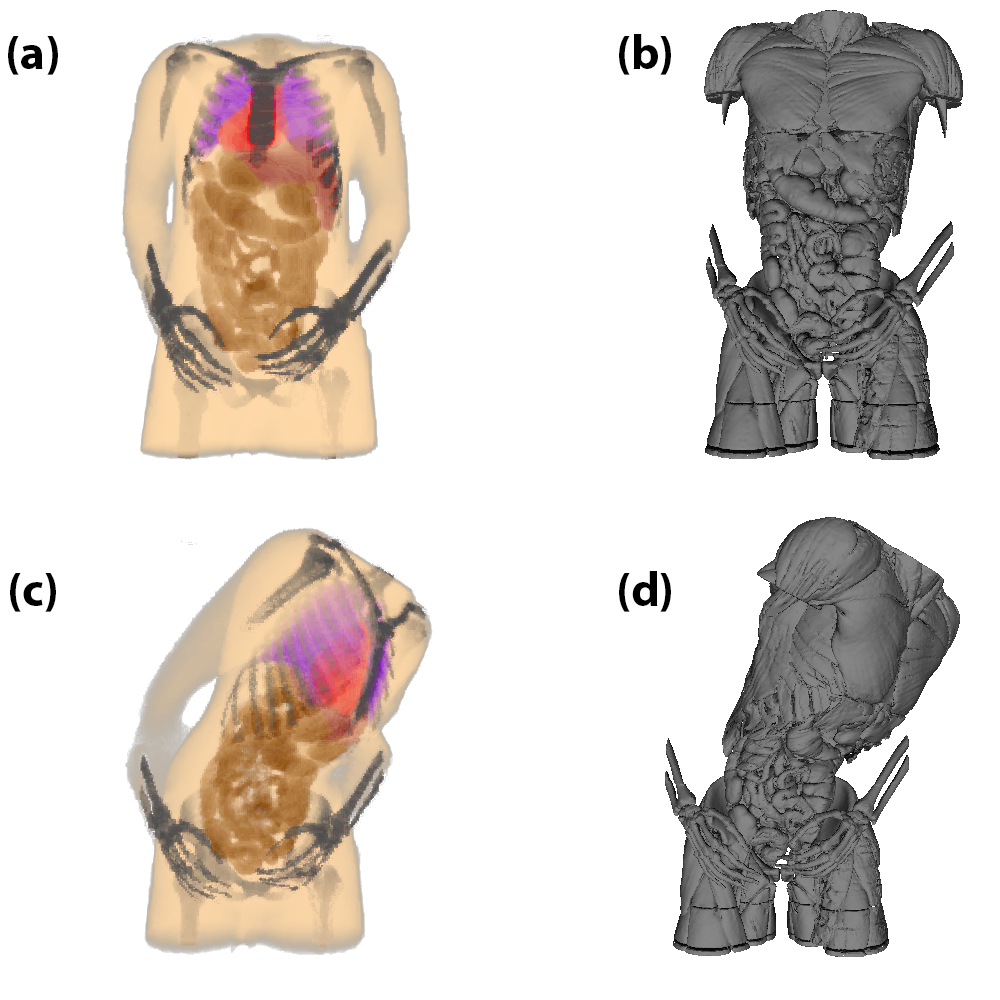
\includegraphics[width=0.4\textwidth]{IMG/HV}
    \caption{Algoritmo aplicado a diferentes representaciones: volumétrica (a) y (c), superficial (b) y (d). Imágenes (a) y (b) muestran el \emph{Segmented Inner Organs} en posición de reposo. Imágenes (c) y (d) muestran el resultado del modelo deformado.}
    \label{fig:humanvisible}
\end{figure}
Con la intención de seguir mostrando las capacidades del algoritmo propuesto, se presentan más ejemplos de deformaciones realizadas para esta tesis. En la figura \ref{fig:humanvisible} se puede observar tanto el modelo superficial como el volumétrico de los datos del modelo \emph{Segmented Inner Organs}(\cite{VM2002},~\cite{VoxelMan}).



%%%%%%%%%%%%%%%%%%%%%%%%%%%%%%%%%%%%% 








%Due to their high content of water, organic tissues can be considered incompressible. For that reason, volume conservation is a desirable feature. In this vein, we have compared the behaviour of LBS, DQS, CoR and our Optimization step (FEM). To this end, we used the same MoCap walk cycle to animate the previously mentioned models. The results of this test are shown in Fig.  \ref{fig:volRatio}.
%\textcolor{red}{It can be observed how the optimization stage solve the volume problems of LBS and DQS. VER QUE PASA CON COR. }
%\begin{figure*}%[!ht]
%   \centering
%    \includegraphics[width=0.98\textwidth]%{img/graficas}
%    \caption{Volumen conservation rate of %the several \emph{skinning} techniques. }
%     \label{fig:volRatio}
%\end{figure*}

\section{Discusión}
\label{posing:discusion}
\todo{Hablar de la necesidad de validación}

\new{A partir de los resultados que se han mostrado en la sección anterior, se puede afirmar que la herramienta puede generar una cantidad infinita de variaciones anatómicas de un mismo modelo anatómico. Además, el cauce diseñado hace que la etapa de selección de poses permita a cualquier usuario animar pacientes virtuales de forma interactiva.}

\new{Hay que remarcar que es necesario una validación formal para comprobar que esta técnica puede ser utilizada en simuladores médicos que en el contexto de entrenamiento puede ser utilizadas para que la transferencia de habilidades de los simuladores que la utilicen sea efectiva. En las siguientes secciones \todo{resultados se moverá al mismo capítulo}, se propondrán dos casos de uso con ese objetivo.}

%\todo{La palabra realista me suena poco cientifica. Plausibles es un resultado que un usuario pueda interpretar como real.  }
%\del{A la vista de los resultados, se puede afirmar que el algoritmo propuesto cumple con la función de generar resultados visualmente \del{realistas}\new{plausible} que en el contexto de entrenamiento puede ser utilizadas para que la transferencia de habilidades de los simuladores que la utilicen sea efectiva. } %\todo{Como puedes afirmar que estos resultados son validos para el entrenamiento!!!!!!!! Has entrenado a médicos y después lo has evaluado!!!!! Aaron cuidado con lo que pones. La hipótesis es esa porque el objetivo era probar este sistema en herramientas reales. Hasta que no haya resultados en un simulador la hipótesis no queda probada!!!!!}

\new{Esta técnica permite generar una cantidad infinita de variaciones anatómicas de un mismo modelo. En cuanto a la variabilidad anatómica ese sentido, este  algoritmo ha sido incorporado en la herramienta \ac{TPTVPH} que va a ser integrada en el \ac{ITGVPH} que tiene como objetivo una base de datos de pacientes virtuales medios que posteriormente podrá ser utilizada en el simulador \ac{RASim}. Esta herramienta podría ser incorporada en otros simuladores que puedan beneficiarse del reposición de modelos anatómicos.}% En el capítulo siguiente, se describirá como se ha incluido la solución presentada en el desarrollo de la herramienta \ac{TPTVPH}.

\new{Por otra parte, con el objetivo de formar parte de herramientas interactivas, este método se puede incorporar en cualquier simulador que requiera cambiar la pose a un determinado modelo anatómico con estructuras internas en tiempo real. Para demostrar esta funcionalidad, se presentará un simulador de radiología diagnóstica que utiliza las ventajas del algoritmo propuesto.}

\new{La técnica de posicionamiento de pacientes virtuales se diseñó con el objetivo de ser lo más flexible posible, minimizando los requisitos de los datos de entrada. La clave de está flexibilidad radica en que se calcula un campo de deformaciones interno. Este campo de deformaciones permite adaptar cualquier tejido a la pose deseada, de forma independiente al resto de tejidos, pudiendo así trabajar con modelos incompletos. En este sentido, la única limitación que se impone es que tanto la piel como el tejido óseo del paciente virtual deben de estar segmentados. Esta restricción no debería suponer un gran problema, dado que estos tejidos son visibles en la mayor parte de las técnicas de imagen médica.}

\new{La flexibilidad que aporta el cálculo del campo interno de deformaciones, aporta beneficios adicionales. Tal y como se muestra en la sección \ref{posing:animvol}, este campo puede aplicarse a estructuras representadas tanto mediante \ac{B-rep}s  como datos volumétricos. Extendiendo de esta manera el alcance de la técnica propuesta. }

\new{Evitar colisiones y autocolisiones en los tejido transformados es de vital importancia de cara a garantizar el buen funcionamiento del simulador físico y del simulador de \ac{US} de \ac{RASimAs}. Con el objetivo de garantizar este requisito, el algoritmo propuesto calcula un campo de deformaciones continuo. De esta forma, solo podrán aparecer colisiones y/o autocolisiones si: (i) se utilizan mallas para representar los tejidos con una resolución inadecuada o (ii) si existen colisiones y/o autocolisiones en el modelo virtual de partida. Debido a que la extracción de los tejidos desde imágenes médicas no es perfecta, pueden aparecer las auto colisiones y colisiones entre tejidos. La técnica propuesta no solventa estas colisiones, pero es robusta en su tratamiento. Aun así, las colisiones con el tejido oseo y muy especialmente con la piel, pueden provocar una importante perdida de realismo. Cabe destacar, que, a pesar de esta circunstancia, la técnica propuesta es mucho más robusta, en este escenario, que los métodos basados en simulación física. En la sección \ref{posing:method}, se proponen técnicas para mitigar estos problemas.
}

\new{ Según los requisitos del proyecto \ac{RASimAs}, la herramienta \ac{TPTVPH} debe permitir a un usuario elegir la postura del paciente virtual de manera interactiva. Además, esta herramienta se podrá configurar con posturas preselecionadas, permitiendo su ejecución de manera completamente automática. Al igual que se muestra en la sección \ref{posing:result}, se pueden cargar poses provenientes de \ac{MoCap} o se pueden guardar posturas manualmente creadas.}

\todo{Esto se va al final de capítulo en la discusión. Lo vamos a meter con las limitaciones de la técnica. }
\new{Por último, se han identificado las siguientes limitaciones:}
\begin{itemize}
    \item Las estructuras mínimas que necesita el algoritmo son la piel y los huesos. Estos tejidos son los más habituales que se pueden capturar en muchas de las imágenes médicas, por tanto, servirán para guiar el proceso e identificar algunos puntos claves para el correcto funcionamiento del algoritmo.
    
    \item Debido a que la extracción de los tejidos desde imágenes médicas no es perfecta, se permiten que haya auto colisiones y colisiones entre tejidos. Aun así, se espera que los diferentes tejidos anatómicos no sobresalgan de la piel, ya que el algoritmo no está diseñado para resolver colisiones, además de no generar colisiones adicionales. Aunque aquellos tejidos que traspasen la piel son irreales, se tratarán por igual aunque no se puede asegurar una deformación realista.
    
    \item El algoritmo utilizará un esqueleto virtual para definir los movimientos de las articulaciones. Se utilizará la información que proporciona los tejidos óseos para construir un esqueleto virtual adecuado al modelo de entrada. La principal limitación es la selección manual de las zonas identificadas que se necesitan para identificar los puntos de rotación de la articulación y su sistema de referencia.
\end{itemize}